\pagebreak
\section{Estado del arte}

Al basarse en los autores consultados, pueden identificar varios conceptos y
técnicas que manejan la ciberseguridad y el mantenimiento preventivo de equipos
de una forma experimental, es decir, que se basan en qué tan efectivas son en
sus campos y se obtuvieron una colección de elementos a tratar. La idea de
tales aportes consiste principalmente en reducir los fallos, ya que como
menciona \textcite{Rathore2023} es imposible que un sistema esté sin errores,
pero es posible reducir su cantidad.

Esto se procura hacer, puesto que independientemente de qué tan sofisticados y
modernos que sean los sistemas de información, siempre se van a encontrar fallas
potenciales y son tan impredecibles como lo son el ver que un equipo deje de
funcionar: ``Dada la necesidad de actualizaciones constantes, la posibilidad de
que se produzcan nuevos fallos en el sistema está siempre presente, con
frecuencia es imprevisible y a veces imposible de prevenir.''
\parencite{Banja2020}

Las revisiones experimentales emplearon técnica que definen el estado actual
del mantenimiento preventivo de equipos tanto de hardware como de software en
la perspectiva de la seguridad, como la extracción de características de un
Malware, el aprendizaje por refuerzo de una inteligencia basada en Machine
Learning, la funcionalidad de un malware, etcétera.

\subsection{Estado de la técnica del mantenimiento preventivo}

Reconociendo los aportes dados por Vieras (2011) como
se cita en \cite{Zambrano2020}, se puede sobreentender el mantenimiento
preventivo como lo que realiza un servicio técnico con los usuarios.

\subsubsection{Machine Learning}

Como tal, su objetivo es automatizar la tarea de construcción de modelos
analíticos para realizar tareas cognitivas como la detección de objetos o la
traducción de lenguaje natural. Esto se consigue aplicando algoritmos que
aprenden iterativamente a partir de datos de entrenamiento específicos del
problema, lo que permite a los ordenadores encontrar ideas ocultas y patrones
complejos sin ser programados explícitamente.
\parencite[Bishop, 2006  como se cita en][]{Janiesch2021}

En la Figura~\ref{fig:venn_diagram} se logra comprender la forma en la
que está constituido el Machine Learning, sobre todo, para distinguer el también 
el llamado Deep Learning que de acuerdo con las mismas fuentes, se considera un
tipo de aprendizaje que requiere de una maquinaria mucho más pesada de lo normal,
es decir que requiere de un coste computacional (memoría, energía y
procesamiento) mucho mayor de lo habitual, por eso es muy común ver su
funcionamiento en servidores y generadores de imágenes:

\begin{displayquote}
  En cambio, los modelos demasiado complejos entrañan un mayor riesgo de
  sobreajuste. Además, su razonamiento es más difícil de interpretar y es
  probable que sean más costosos desde el punto de vista informático. Los
  costes computacionales se expresan mediante los requisitos de memoria y el
  tiempo de inferencia para ejecutar un modelo en datos nuevos. Estos criterios
  son especialmente importantes a la hora de evaluar las redes neuronales
  profundas, en las que pueden procesarse y almacenarse varios millones de
  parámetros del modelo, lo que impone exigencias especiales a los recursos de
  hardware. \parencite{Janiesch2021}
\end{displayquote}

\begin{figure}[htb]
  \centering
  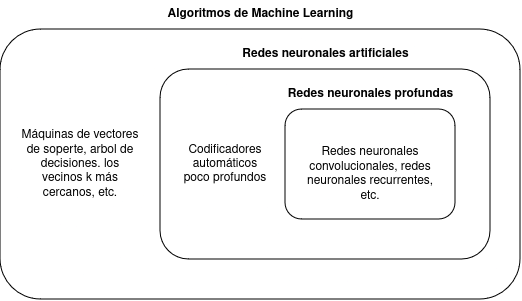
\includegraphics[width=0.75\textwidth]{./pictures/venn_diagram.png}
  \caption{
    \textbf{Nota:} Diagrama de Venn de los conceptos y clases del Machine
    Learning. Tomado de \cite{Janiesch2021}
  }
  \label{fig:venn_diagram}
\end{figure}

Para describir cómo funciona, \textcite{Janiesch2021} comentan que esta
inteligencia se utilizan las tres técnicas fundamentales en donde se aplica su
uso: ``En función del problema planteado y de los datos disponibles, podemos
distinguir tres tipos de Machine Learning: aprendizaje supervisado, aprendizaje
no supervisado y aprendizaje por refuerzo.''

\begin{itemize}
  \item \textbf{Aprendizaje supervisado:}
    Por norma general, \textcite{Janiesch2021} lo definen como una serie de datos
    preexistentes los cuales le sirven a la inteligencia para tener criterio tanto
    de elementos de entrada, como de salida de un sistema que muchas veces es un
    software que se dedica a recopilar información; por ejemplo, de una base de
    datos que almacena suscripciones de un sitio web cualesquiera.

  \item \textbf{No supervisado:}
    Esta técnica en el contexto de intentar encontrar anomalías en un sistema
    individual o un conjunto de estos, se refiere como la detección de patrones
    sin necesidad de información a priori y al aprendizaje se realiza al
    identificar un ``factor común'' de grupos que conforman la información que la
    inteligencia recibe: ``Machine Learning se define como ``la adquisición de una
    descripción estructural a partir de ejemplos''. Esta descripción puede
    utilizarse para inferir reglas de clasificación (u otro tipo de reglas no
    supervisadas, por ejemplo, reglas de agrupación)''.
    \parencite[Witten et al., 2011, como se cita en][]{Singh2022}

  \item \textbf{Aprendizaje por refuerzo:}
    Cuando la inteligencia está con cierto grado de criterio gracias al aprendizaje
    supervisado y con la funcionalidad implementada en el aprendizaje no
    supervisado, se utiliza entonces el aprendizaje por refuerzo para poder ampliar
    nuevos conocimientos y habilidades a través de ``recompensas'' y ``castigos'',
    los cuales hacen que la inteligencia tenga una mejor toma de decisiones:

    \begin{displayquote}
      El aprendizaje por refuerzo funciona secuencialmente en un entorno
      realizando una acción, evaluando su recompensa y ajustando las acciones
      siguientes en consecuencia. En concreto, un paradigma de aprendizaje por
      refuerzo implica un agente que observa el entorno y realiza acciones para
      maximizar la recompensa determinada por el problema en cuestión.
      \parencite[Richard S Sutton y Andrew G Barto., 2018, como se cita en][]
      {Chen2023}
    \end{displayquote}

    Los mismos autores mencionan otros elementos clave relacionados con el
    aprendizaje bajo refuerzo tales como el espacio de acción, entorno, estado,
    observaciones y recompensa y política. El espacio de acción se refiere a las
    opciones que puede tomar el agente por medio inteligencia gracias al
    aprendizaje supervisado. \parencite{Janiesch2021}

    El entorno se considera el espacio en donde se puede mover el agente. El
    estado se refiere a las condiciones en las que se presenta el mismo a modo
    de configuración. La recompensa se refiere al mayor beneficio que se puede
    obtener a nivel tras realizar las acciones que se obtienen en el entorno. Y
    la política significa que, dado un estado, la inteligencia por medio del
    agente ha de realizar una serie acciones específicas de acuerdo con sus
    posibilidades. \parencite{Chen2023}
\end{itemize}

\iffalse
\subsubsection{Manejo de dispositivos de IoT}

% mmejorar esta parte

IoT (Internet de las cosas, en inglés) a pesar de no ser una parte muy común,
cada vez en el ámbito tecnológico se vuelve importante, ya que hace un cambio
radical respecto a cómo nos comunicamos y cómo transmitimos la información. 
\textcite{Singh2022} comenta que 
\fi

\subsubsection{Ada Test}

El fundamento de poder explicar lo que es Ada Test, primero 
define los siguientes conceptos conceptos:


Ada test, \textcite{Chen2023} se muestra como un algoritmo de pruebas sobre la
existencia de troyanos de hardware, dicho algoritmo pasa por las siguientes
fases: Fase I (Perfilado de circuitos), Fase II (Generación de patrones de
prueba adaptativos basados en aprendizaje por refuerzo). Tal algoritmo se
propuso como una mejora a los métodos que se emplean para estudiar el estado de
los circuitos integrados de forma que cuando se estén utilizando, se emplee su
desempeño como corresponde, que sea seguro para procesadores de sistemas de
cómputo y que no implique desarmar el circuito para comprobar su funcionamiento.
La manera en como se conoce esto, es a través de los siguientes conceptos que 
\textcite{Chen2023} explicó:

\begin{itemize}
  \item \textbf{Troyano de hardware:}
    Modificaciones maliciosas en el hardware que pueden encontrarse por defecto
    en la cadena de los circuitos integrados de una máquina. Normalmente tiene
    dos características: Payload y gatillo, la primera consiste el efecto del
    circuito que no funciona como debería y la segunda es la señal que determina
    si la payload se ejecutará o no. La Figura~\ref{fig:circuit} utiliza un
    circuito con puertas lógicas AND y XOR que son usadas para gatillo y
    payload respectivamente.

  \item \textbf{Puertas lógicas:}
    Para conocer lo que ocurre en la Figura~\ref{fig:circuit}, tenemos que
    asumir que desde el lado izquierdo, está circulando corriente eléctrica en
    una o más líneas del esquema, que resultan ser las entradas de las puertas
    lógicas; es irrelevante saber por dónde entra la corriente, pues lo
    importante es saber que las puertas lógicas son componentes electrónicos
    que definen si la corriente continua a través de ellas o no. La forma en la
    cual estas puertas definen las decisiones, se basan directamente en
    operadores lógicos en matemáticas (por ejemplo, las puertas AND se
    comportarán como el operador de conjunción, el OR se comportará como el
    operador de disyunción, etc). La Figura~\ref{fig:logic} expresa el
    funcionamiento de tales puertas.

  \item \textbf{Análisis de canal lateral:}
    Es la revisión de troyanos de hardware para determinar si hay un cambio en
    los parámetros físicos (como energía o retarde del trayecto del circuito)
    y para conocer su presencia se utiliza un esquema de circuito bajo prueba
    para comprobar si el troyano directamente hace una modificación en el
    circuito.

  \item \textbf{Pruebas lógicas:}
    Puede detectar troyanos funcionales, es decir aquellos que eliminan y añaden
    otras operaciones de bajo nivel; cambia la funcionalidad básica de las
    operaciones lógicas. El problema de las pruebas lógicas es que involucra
    dejar ciertos caminos que pueden implicar otros circuitos de troyanos de
    hardware parecidos a los de Figura~\ref{fig:circuit}

  \item \textbf{Perfilado de circuitos}
    Es una fase de Ada Test en donde se computa la transición de probabilidades
    de cada nodo y se computa los parámetros de capacidad de prueba del programa
    de Análisis de Controlabilidad/Observabilidad Sandia. Esta fase busca
    principalmente generar un circuito bajo pruebas con el fin de determinar si
    un circuito puede tener troyanos de hardware de la manera en como se espera.

    Computar la transición de probabilidades en cada nodo (puerta lógica) de la
    lista de redes implica en reconocer los elementos de un troyano de hardware
    del mismo. Para realizar tal computación se utiliza un modelo matemático tal
    que así: $ P_{trans} = p(1-p) $ donde $ p $ es resultado de la probabilidad
    de cada nodo y $ P_{trans} $ es comparado con un umbral $ \theta $ para
    encontrar los nodos ``raros'', los cuales identifican tanto las payloads
    como los gatillos del troyano.

    Y computar los parámetros de capacidad de prueba del programa de Análisis de
    Controlabilidad/Observabilidad Sandia comprueba la calidad de los nodos
    raros; la controlabilidad describe la habilidad de establecer un valor
    específico de un nodo. La observabilidad consiste en determinar los valores
    de un nodo controlando sus entradas y comprobando su salida\dots algo muy
    similar a la comprobación de la secuencia de arranque de las placas madre
    modernas.
  \item \textbf{
      Generación de patrones de prueba adaptativos basados en aprendizaje por
      refuerzo}
    En esta fase, Ada Test realiza una generación de prueba de entrada. Para
    ello, se genera un conjunto de vectores iniciales de prueba, luego se
    genera una serie de patrones candidatos que podría mejorar la detección del
    rendimiento cuando se añade al conjunto de pruebas, posteriormente Ada Test
    por medio del aprendizaje por refuerzo aprendido por \textcite{Janiesch2021}
    para comprobar su funcionalidad (qué tan alta es su calidad) de cada prueba.

    Esto se hace principalmente para obtener un mayor grado de conocimiento
    sobre los troyanos de hardware de una manera más limpia.
\end{itemize}

Lo que significa que para el mantenimiento preventivo de un equipo, se puede
sacar provecho a los algoritmos de las inteligencias artificiales (sobre todo
Machine Learning con aprendizaje por refuerzo) para realizar una mejor
comprensión del estado tanto del hardware como del software.

\begin{figure}[htb]
  \centering
  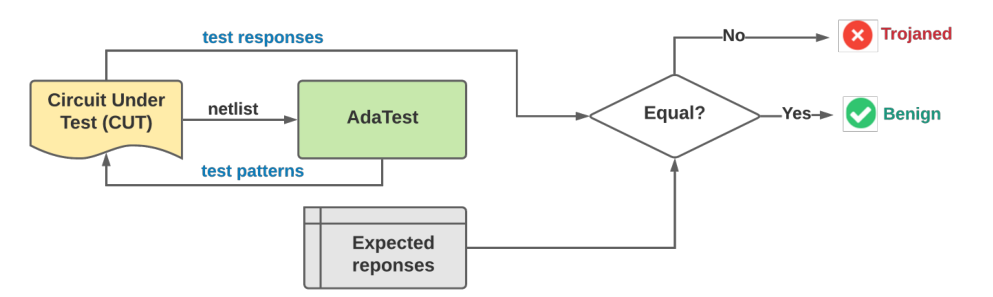
\includegraphics[width=0.75\textwidth]{./pictures/adatest.png}
  \caption{
    \textbf{Nota:} Circuit Under Test (Circuito bajo prueba), Expected responses
    (Respuestas esperadas), Test responeses (Prueba de respuestas) y Test
    patterns (Pruebas de patrón) son los elementos y sus salidas en inglés de
    la representación de Ada Test. Tomado de \cite{Chen2023}}
  \label{fig:adatest}
\end{figure} 

\begin{figure}[htb]
  \centering
  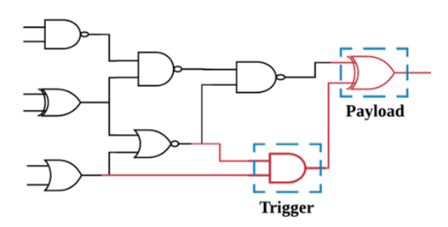
\includegraphics[width=0.75\textwidth]{./pictures/circuit.png}
  \caption{
    \textbf{Nota:} Este esquema es la demostración de un troyano de hardware.
    Tomado de \cite{Chen2023}}
  \label{fig:circuit}
\end{figure} 

\begin{figure}[htb]
  \centering
  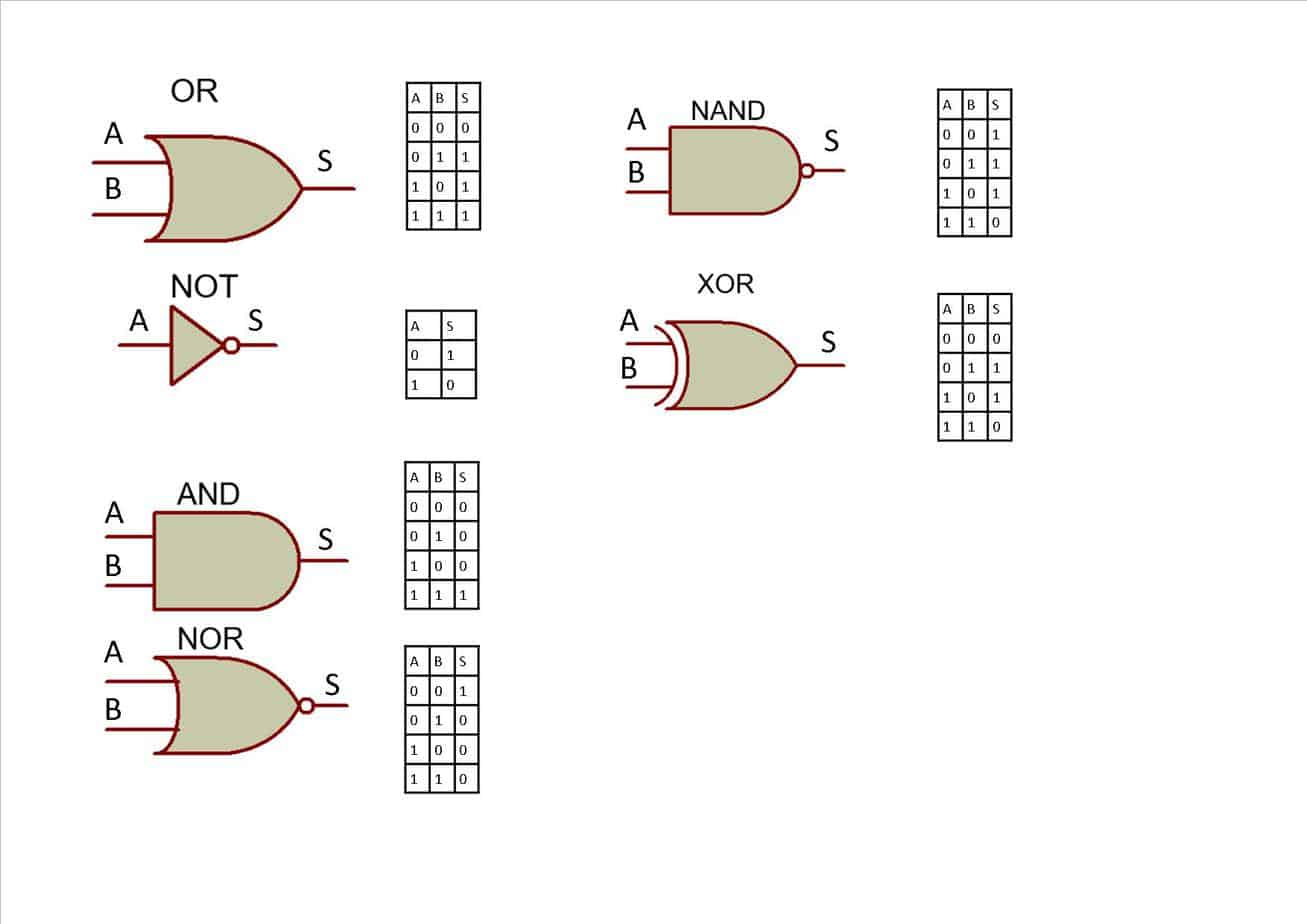
\includegraphics[width=0.75\textwidth]{./pictures/logic.png}
  \caption{
    Colección de las puertas lógicas y sus operaciones básicas dependiendo de la
    entrada que se le designe.
  }
  \label{fig:logic}
\end{figure} 

\subsection{Estado de los elementos de la ciberseguridad}

La manera en como se logra ver los conceptos de ciberseguridad, lo describe
\textcite{Mosquera2019} cuando trata de referirse a reducir los fallos que
puedan presenciarse gracias a las amenazas de la información de un activo (en
el contexto empresarial, se suele referir a los sistemas informáticos que
pertenecen a una organización y que pueden ser variados):
``La protección de activos de información, a través del tratamiento de amenazas
que ponen en riesgo la información que es procesada, almacenada y transportada
por los sistemas de información que se encuentran interconectados''
\parencite[Esic Business \& Marketing School, 2020, como se cita en][]{Bueno2022}

\subsubsection{
  Riesgos de seguridad e inteligencia artificial en los sistemas de salud
}

Por lo que se sabe, se piensa que cuando se tiene que implementar un sistema
inteligente, independientemente del tipo que sea, se sabe que puede ser
extremadamente útil para radiografías o identificación de patologías, pero se
sabe que esto puede conllevar a fallas desastrosas si se deja alguna brecha que
puede aprovechar un malware que rompa la cadena que lleva la red neuronal que
se emplea:

\begin{displayquote}
  Cabe recordar el artículo de 2010 de Dudzinski y sus colegas en el que se
  examinaban fallos puntuales -como lagunas en el control de infecciones, mal
  funcionamiento de la tecnología de desinfección, errores de laboratorio y
  clínicos incompetentes- que llegaron a afectar a miles de pacientes.
  \parencite{Banja2020}
\end{displayquote}

A esto se le suma al hecho de que también se puede añadir otros propósitos a la
información crítica de los usuarios, es decir, que se puede tomar esos datos
para utilizarlos para otros fines en lugar de los que son puestos.
\parencite{Banja2020}

\subsubsection{Manejo Legislativo}

Uno de los intentos que se realizaron a nivel nacional, fue el de mitigar los
ciberataques por medio de las normas del código penal colombiano, las cuales
condenan varias de las técnicas de ataque que afectan a los ciudadanos las
cuales incluyen suplantación de sitios web, robo de datos, hurto por medios
informáticos y otros delitos tratados por la ley. \parencite[Ley 1273 de 2009.
Por medio de la cual se modifica el Código Penal, se crea un nuevo bien jurídico
tutelado - denominado “de la protección de la información y de los datos”- y se
preservan integralmente los sistemas que utilicen las tecnologías de la
información y las comunicaciones, entre otras disposiciones. 5 de enero de 2009.
D.O. No. 47223, como se cita en][]{Mosquera2019}

Añadido a esto, nacionalmente se encontraron otras soluciones que se llevan
haciendo desde la popularización de la informática a nivel nacional, como por
ejemplo de que en las empresas se intente fomentar la seguridad de los equipos
pese a las circunstancias que se estén manejando para prevenir fallos en los
sistemas de información:

\begin{displayquote}
  Aparte de estos avances paulatinos, también debe tenerse en cuenta que en el
  transcurso de todo el año 2021, el Ministerio TIC, se empeñó en capacitar
  gratuitamente a PyMES (Pequeñas y Medianas Empresas) en materia de
  ciberseguridad, esto con el fin implementar acciones para proteger la
  información y para lograrlo era necesario que sus equipos de trabajo
  estuvieran en capacidad de enfrentar este reto y dar respuesta inmediata a
  cualquier tipo de amenaza.
  \parencite[MinTic, 2021, como se cita en][]{Bueno2022}
\end{displayquote}

\subsubsection{Tipos de malware}

En las revisiones de \textcite{Mosquera2019} se identificó la importancia de
hacer una revisión de los especímenes de malware a los que los servidores y
sistemas de cómputo individuales son atacados constantemente. Esto se hace,
puesto que esta situación por lo general, obliga a los desarrolladores a poner
mayor énfasis en la protección ante ciertos tipos de entradas maliciosas que
generan vulnerabilidades.

\begin{itemize}
  \item \textbf{Gusano:}
    Es semejante a un virus, la diferencia radica en que este se replica tanto
    en otro software como en la red sin necesidad de la supervisión de un
    usuario. \parencite{Rosli2019}

  \item \textbf{Troyano:}
    Es un malware que se presenta como un software legítimo; cumple la función
    de virus o gusano, solo que su principal fundamento es el uso del engaño de
    tal forma que un usuario piense que está usando un programa legítimo.
    \parencite{Rosli2019}

  \item \textbf{Botnet:}
    Es una red de computadoras infectadas, tales computadoras se les llaman
    ``bots'' los cuales cumplen las finalidades de un atacante, el cual logra
    acumular varios de estos ``bots'' a través troyanos o gusanos: ``Botnet
    también se define como una colección de ordenadores que han sido infectados
    por software malicioso y los convierte en bots, drones o zombis, que se han
    integrado en una colección mayor a través de una infraestructura
    centralizada de mando y control.'' \parencite{Rosli2019}

  \item \textbf{Ransomware:}
    Este tipo de malware busca encriptar toda la información en una máquina y
    luego hacer que el usuario inserte una clave para desencriptarla; las claves
    dadas por los atacantes requieren de una demanda otorgada por ellos, como
    pedir una cierta cantidad de dinero: ``Normalmente, una máquina infectada
    por ransomware queda ``congelada'', ya que el usuario no puede abrir ningún
    archivo, y la imagen del escritorio se utiliza para proporcionar información
    sobre las demandas de los atacantes.'' \parencite{Rosli2019}

  \item \textbf{Spyware:}
    Como su nombre lo dice, es un malware que se dedica a seguir al usuario de
    tal forma que este último no se dé cuenta del hecho. Se dedica
    principalmente a revisar los historiales de búsqueda, monitorear las
    actividades (para luego venderlas a terceros).
    \parencite{Rosli2019}
\end{itemize}

\subsubsection{Técnicas comunes de hacking}

% Insertar un parrafo introductorio a estas técnicas
% Meter otros conceptos

\begin{itemize}
  \item \textbf{Phishing:}
    Cuando una persona recibe un correo electrónico en el que un atacante se
    muestra como alguien importante, por norma general tienden a tentarse
    principalmente en hacer caso a las peticiones que se dan de tal forma que
    puedan aprovecharse del descuido generado por parte de los usuarios. Puede
    presentarse como un correo que hace una petición de credenciales, para que
    accedan a una página web de dudosa procedencia o para descargar malware
    asegurando que es solo un archivo de texto. De esa manera se logra ingresar al
    dispositivo de un usuario que la mitad del tiempo es incauto al llevarse por la
    impresión que genera el correo:

    \begin{displayquote}
      El delito con mayor crecimiento en el 2021, fue la violación de los datos
      personales, con un crecimiento de aproximadamente el 45\% con respecto al 2020,
      mediante la modalidad llamada ``phishing'' donde los cibercriminales realizan
      envíos masivos de emails adjuntando enlaces a páginas webs fraudulentas, así
      pueden llegar a infectar el dispositivo con un archivo adjunto malicioso o
      ``malware'' y de esta manera roban la información que necesitan.
      \parencite[INCIBE, 2010, como se cita en][]{Bueno2022}
    \end{displayquote}

    \iffalse
  \item \textbf{Ataques DDoS:}
    Chingar un equipo gigante que está para servir a montones de usuarios
    \fi

  \item \textbf{Vishing:}
    También conocido como el tráfico de datos personales, en este tipo de
    técnicas no se requiere de un malware, porque lo fundamental de esta
    técnica es el uso de la ingeniería social (engaño) para obtener información
    personal para ganar un beneficio monetario a través de sus datos.
    \parencite{Mosquera2019}

  \item \textbf{Uso de pirámides:}
    No se refiere literalmente a los polígonos tridimensionales, se refiere a
    una representación virtual de una estafa piramidal. Esto se logra sabiendo
    que en las criptomonedas hay incertidumbre en la legalidad y fluctuación,
    por lo que los inversionistas poco cuidadosos eventualmente compran una
    moneda virtual a unos estafadores que presumen ser expertos en tal economía.
    \parencite{Mosquera2019}

  \item \textbf{Suplantación de correo corporativo:}

  \item \textbf{Carding:}
    Como se intuye por el nombre, se refiere al robo de los datos de tarjetas de
    crédito o de débito, también con respecto a información financiera como las
    cuentas bancarias de una persona. Este tipo de técnicas se divide en varios
    métodos para obtener información, como el ``skimming'', el cual se resume en
    la clonación de tarjetas. \parencite{Mosquera2019}

  \item \textbf{Ofuscación:}
    Cuando se trata de leer un código de malware, para pasar desapercibido por
    un usuario, lo que se hace es ofuscarlo. Ofuscar un archivo significa
    modificarlo de tal forma que no pueda ser legible para cualquier usuario,
    esto a pesar de pasar desapercibido por cualquier usuario y antivirus, sigue
    siendo funcional cuando se ejecuta.
    \begin{displayquote}
      La imagen de memoria basada en opcodes puede tomarse para representar
      dinámicamente las actividades maliciosas. Aunque el malware ofuscado no
      puede ocultar cómo se comporta cuando se analiza dinámicamente, el
      análisis dinámico es incapaz de satisfacer todas las condiciones
      maliciosas para explorar todas las rutas de ejecución.
      \parencite{Aboaoja2022}
    \end{displayquote}
\end{itemize}

\subsubsection{Intentos de estudiar el malware}

Conociendo que cada vez se mejora la seguridad de los equipos de cómputo,
\textcite{Aboaoja2022} comenta que también se busca crear software malicioso que
realice sus funciones mientras no sea detectado. Por ende, para conocer las
funciones que realiza el programa, se realiza un proceso de análisis que se
caracteriza por tener tres tipos de acercamiento: Estático, dinámico e híbrido:
El primero consiste en estudiar el malware sin ejecutarlo, el segundo es
ejecutarlo para comprobar su comportamiento y el tercero, es usando las ventajas
que ofrecen los dos anteriores de acuerdo a los contextos (si el malware no
se puede analizar sin ejecutarlo, se puede usar el análisis dinámico, pero
siempre en un entorno que no esté conectado a internet y no cuente con
información crítica del usuario)

Estos tipos de análisis logran obtener ciertos tipos de datos, en los cuales se
puede tomar en consideración la metodología de análisis más correcta de acuerdo
a una situación en particular; por ejemplo, si se tiene un malware que realiza
una serie de llamadas API, resulta más conveniente usar el análisis dinámico,
ya que por medio de este se logra comprender directamente cuáles son las
herramientas del sistema que tiene por defecto. Del mismo se aplica para
archivos que están pensados para escalar privilegios dentro del sistema, como lo
pueden ser las bibliotecas de enlace dinámico (archivos con código ejecutable
que se cargan según la necesidad de un programa) o archivos portables (la
estructura más común para archivos ejecutables)
\parencite{Aboaoja2022}

Aparte de estos modelos de análisis de malware, lo que se necesita evidentemente
antes de provocar errores inesperados por parte de la operación de algún
malware, lo que se hace dependiendo del tipo de malware es usar unos modelos de
detección. Estos modelos son basados en firma, comportamiento, heurístico y
discusión. \parencite{Aboaoja2022}

A continuación, se hace una descripción de tales modelos según la información
otorgada por los mismos autores:

\begin{itemize}
  \item \textbf{Modelo basado en firma}
    El modelo basado en firma, consiste en encontrar un patrón muy común en
    archivo con código ejecutable, es muy frecuente que sea automatizado por
    los programas antivirus, ya que estos comparan las firmas que tienen según
    la base de datos en donde se encuentra vinculados para evitar más
    comportamientos semejantes.

  \item \textbf{Modelo basado en comportamiento}
    Como bien se intuye, lo que se hace es ejecutar el código del malware en un
    entorno asegurado, concretamente en una máquina virtual. Las máquinas
    virtuales son simuladores de sistemas operativos completamente funcionales,
    pero cuya información no está relacionada con la del disco duro del usuario.

  \item \textbf{Modelo basado en heurística}
    Una vez extraída la información, lo que se hace primero es generar una
    serie de reglas genéricas que pueden ser también generadas por una
    inteligencia artificial (La herramienta YARA realiza tales acciones
    basándose en los aprendizajes no supervisados de Machine Learning). Luego
    con esas reglas, se investiga el contenido del malware empleando las
    técnicas estáticas y dinámicas.

  \item \textbf{Modelo basado en discusión}
    Como las desventajas de los análisis del malware se hacen presentes al
    aplicarlos en archivos con código ofuscado y con comportamientos poco
    predecibles, se considera entonces que es una situación en discusión. En
    otras palabras, las técnicas a emplear no son suficientes para conocer las
    características del malware y se tienen que descubrir para realizar otras
    acciones.
\end{itemize}

\subsubsection{Líneas de tiempo acorde a los tópicos}

\begin{figure}[hb!]
  \centering
  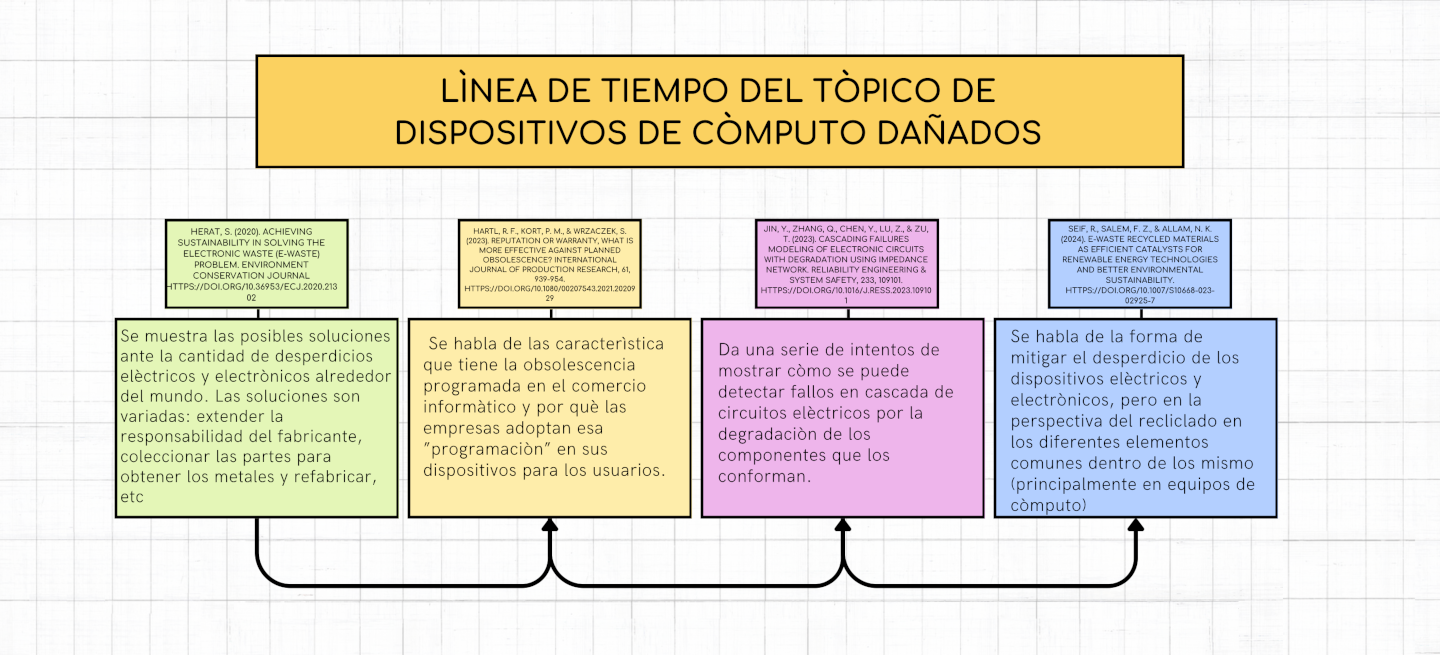
\includegraphics[width=1\textwidth]{./pictures/timeline_1.png}
  \caption{Línea de tiempo del tópico de dispositivos de cómputo dañados}
  \label{fig:timeline1}
\end{figure} 

\begin{figure}[ht!]
  \centering
  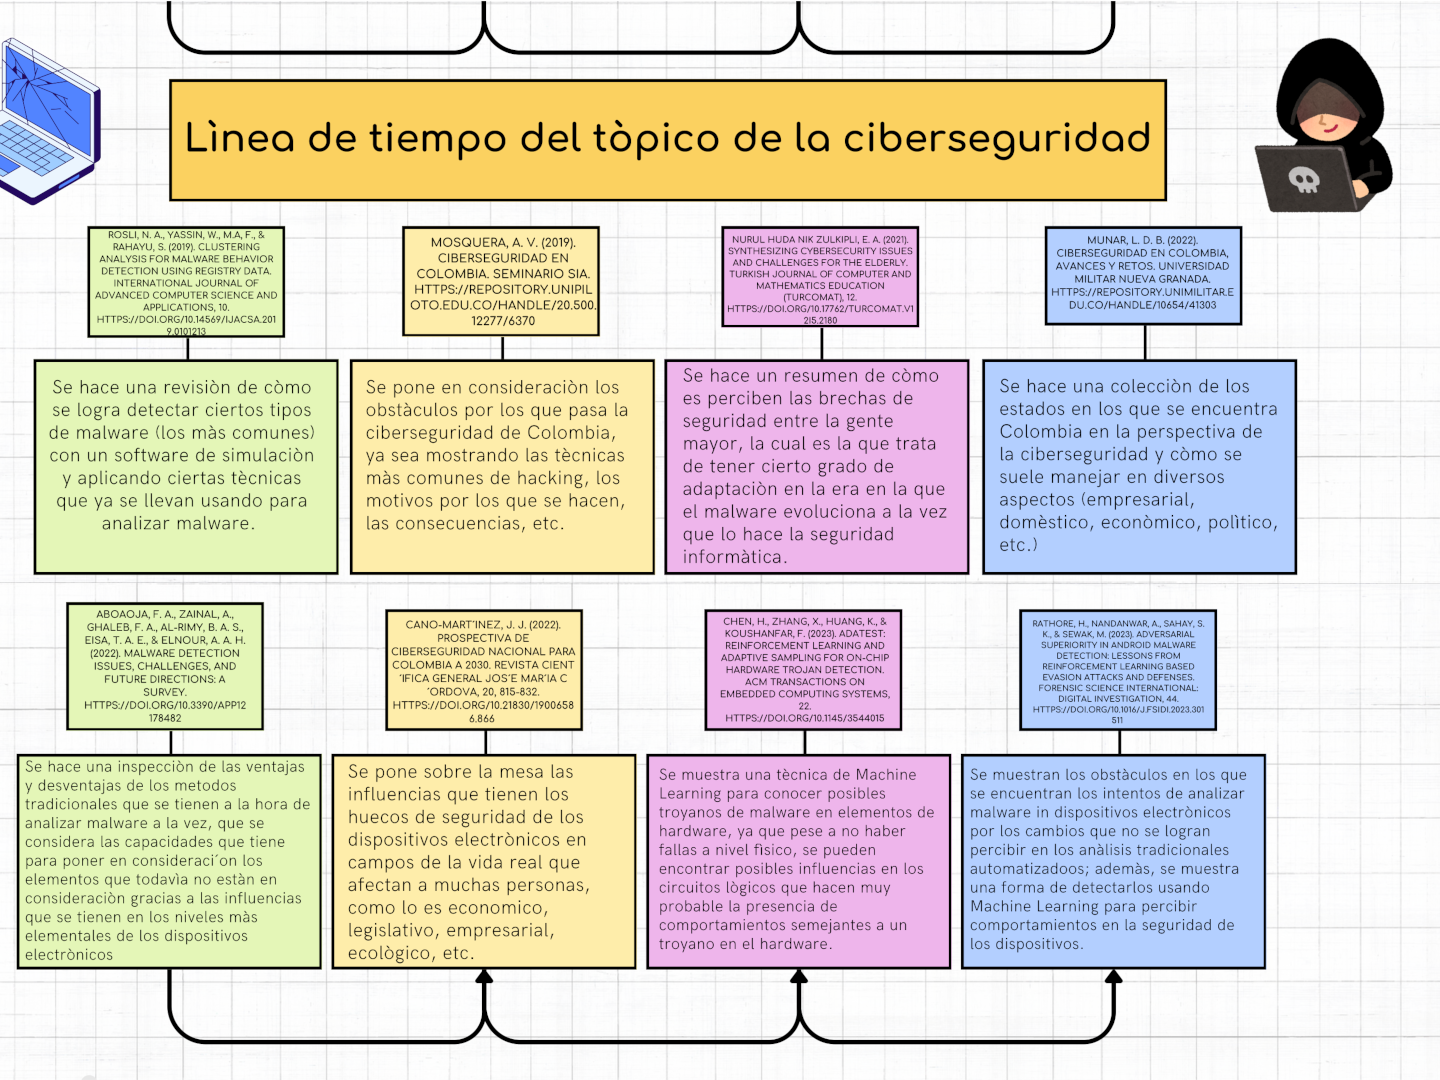
\includegraphics[height=0.5\textheight]{./pictures/timeline_2.png}
  \caption{Línea de tiempo del tópico de la ciberseguridad}
  \label{fig:timeline2}
\end{figure} 

\begin{figure}[hb!]
  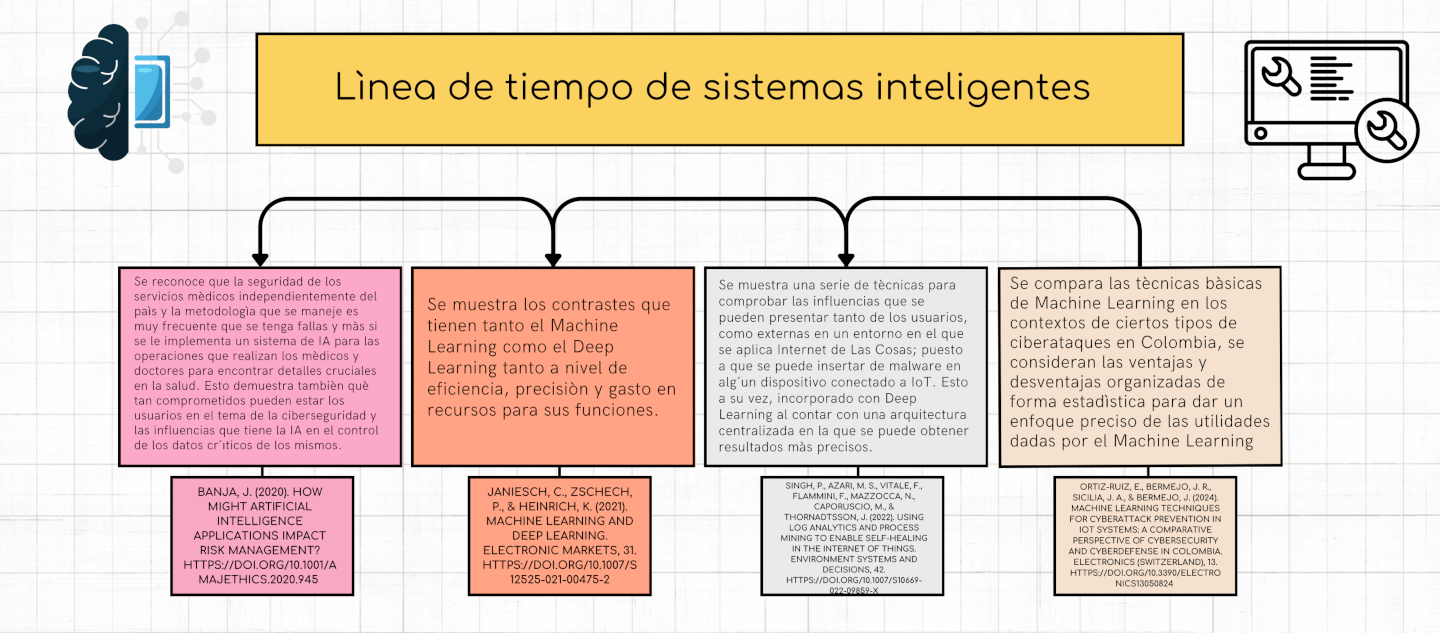
\includegraphics[width=0.85\textwidth]{./pictures/timeline_3.png}
  \caption{Línea de tiempo de sistemas inteligentes}
  \label{fig:timeline3}
\end{figure} 

\begin{figure}[ht!]
  \centering
  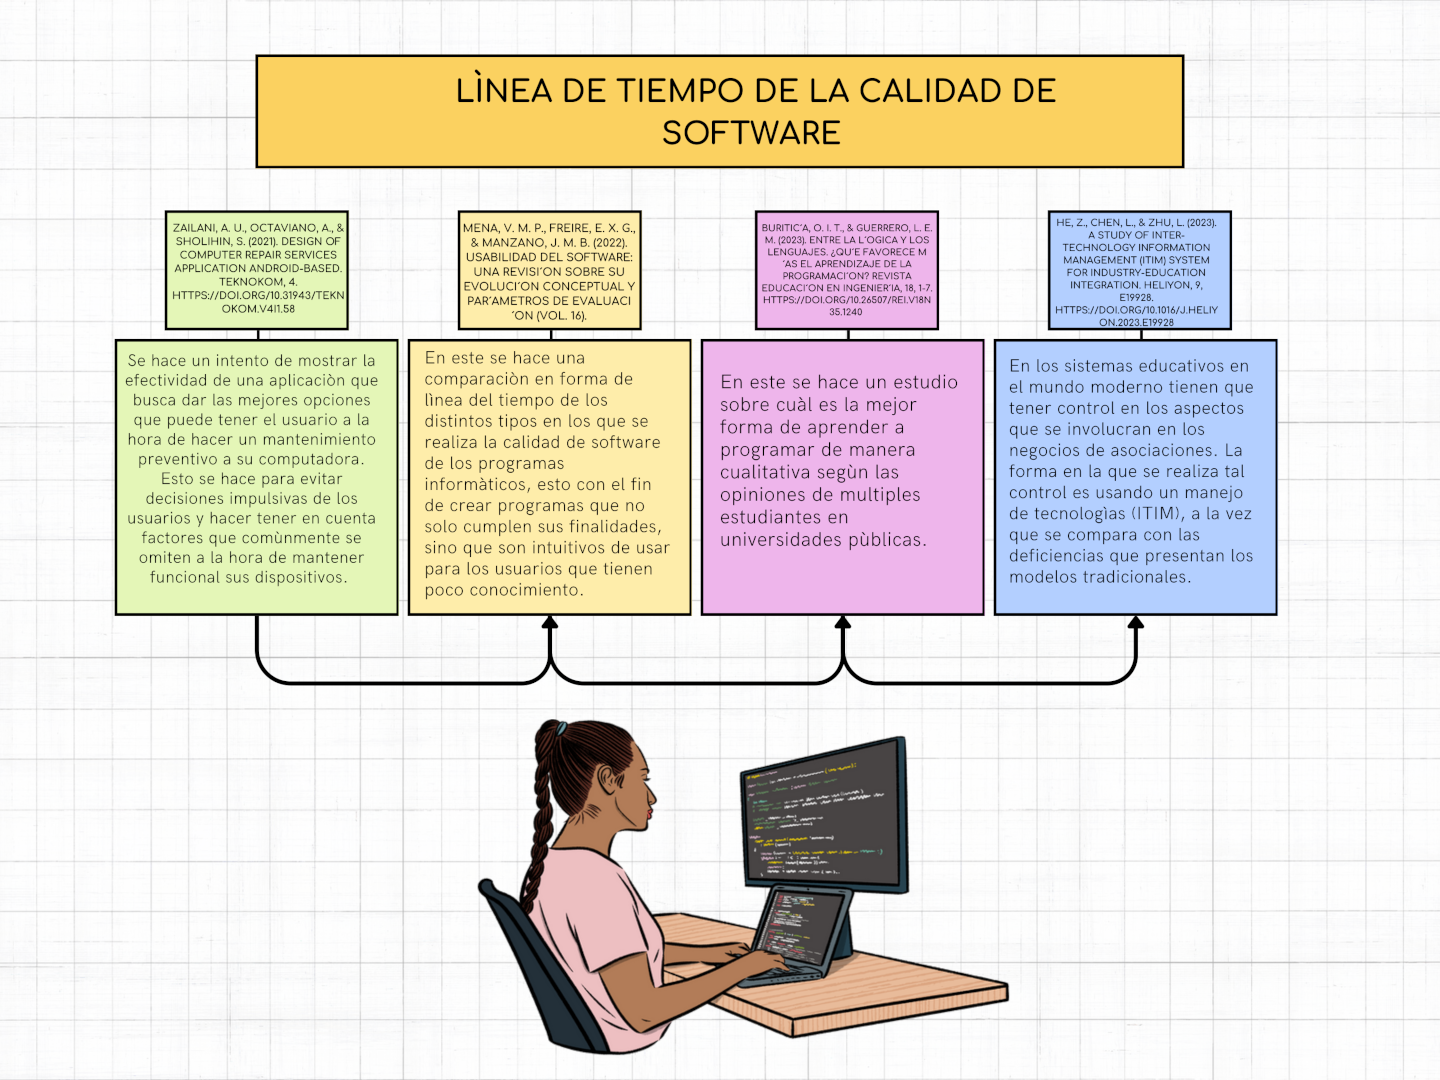
\includegraphics[width=1\textwidth]{./pictures/timeline_4.png}
  \caption{Línea de tiempo de la calidad de software}
  \label{fig:timeline4}
\end{figure} 
